\documentclass[12pt,a4paper]{article}
\usepackage[utf8]{inputenc}
\usepackage[T1]{fontenc}
\usepackage[spanish]{babel}

% Tipografía y espaciado compacto
\usepackage{microtype}
\usepackage{setspace}
\setstretch{0.95}
\setlength{\parskip}{0pt}
\setlength{\parindent}{1em}

% Márgenes reducidos
\usepackage{geometry}
\geometry{a4paper, margin=0.75in}

% Matemáticas y gráficos
\usepackage{amsmath,amssymb}
\usepackage{graphicx}
\usepackage[font=small,labelfont=bf,skip=4pt]{caption}

% Tablas eficientes
\usepackage{booktabs}
\usepackage{array}
\newcommand{\tablesmall}{\scriptsize}

% Control de flotantes
\usepackage{float}
\setlength{\textfloatsep}{8pt plus 1pt minus 2pt}
\setlength{\floatsep}{6pt plus 1pt minus 1pt}
\setlength{\intextsep}{6pt plus 1pt minus 1pt}

% Espaciado compacto en secciones
\usepackage[compact]{titlesec}
\titlespacing*{\section}{0pt}{2.5ex plus 0.5ex minus .2ex}{1ex plus .2ex}
\titlespacing*{\subsection}{0pt}{2ex plus 0.5ex minus .1ex}{0.8ex plus .1ex}

% Enlaces y metadatos PDF
\usepackage[
    pdftitle={Proyecto de Ampliación: Planta Ensambladora de Motocicletas},
    pdfauthor={Juan Andrés Rojas – Esteban Ibarra},
    pdfsubject={Álgebra Lineal Aplicada},
    pdfkeywords={Mínimos Cuadrados, Regresión Lineal, Pronóstico de Demanda, Planificación de Inventario},
    bookmarks=true,
    bookmarksopen=true,
    colorlinks=true,
    linkcolor=blue,
    citecolor=blue,
    urlcolor=blue
]{hyperref}

\title{\vspace{-1cm}
    Proyecto de Ampliación: Planta Ensambladora de Motocicletas \\
    \large Pronóstico de Demanda y Planificación de Inventario Mediante Mínimos Cuadrados y Análisis de Incertidumbre
}
\author{
    Juan Andrés Rojas – Esteban Ibarra \\
    Universidad Tecnológica \\
    Curso de Álgebra Lineal \\
    $2^{\text{o}}$ Semestre
}
\date{Mayo 27, 2025}

\begin{document}

\maketitle
\thispagestyle{empty}

\begin{abstract}\small
Este trabajo utiliza el método de mínimos cuadrados para \textbf{pronosticar la demanda y planificar el inventario} de MotoTec. A partir de datos históricos de ventas (2013–2022) de cuatro tipos de motocicletas, se proyectan ventas (2023–2027) y se estiman necesidades de componentes. Incluye métricas de ajuste (ECM, R²), un \textbf{modelo global (hiperplano)}, \textbf{intervalos de predicción} y una \textbf{simulación de Monte Carlo} para analizar incertidumbre. El repositorio con el código completo está en GitHub.
\end{abstract}

\section{Introducción}
MotoTec enfrenta volatilidad en la demanda y alta dependencia de componentes importados (70\% de Asia). El objetivo es \textbf{reducir inventario en un 25\%} sin afectar producción. Aplicamos \textbf{métodos de mínimos cuadrados} para:
\begin{enumerate}
    \item Pronosticar ventas de cuatro familias de motos (urbanas, turismo, off-road, eléctricas) para 2023–2027.
    \item Calcular necesidades de 10 componentes clave por año.
    \item Cuantificar incertidumbre mediante un \textbf{modelo global} y \textbf{simulación de Monte Carlo}.
\end{enumerate}

\section{Marco Teórico}
\subsection{Matriz y Mínimos Cuadrados}
Una \textbf{matriz} $A$ organiza datos (ventas vs.\ tiempo). El método de \textbf{mínimos cuadrados} resuelve
\[
A\mathbf{x} \approx \mathbf{b}
\]
minimizando la suma de cuadrados de residuos. Si $A^T A$ es invertible, la solución es
\[
\mathbf{x}^* = (A^T A)^{-1} A^T \mathbf{b}.
\]
Si no lo fuera, se emplea la \textbf{pseudoinversa de Moore–Penrose} $A^+$.

\subsection{Regresión Lineal Simple}
Modelamos las ventas $S(t)$ como
\[
S(t) \;=\; \beta_0 + \beta_1\,t,
\]
donde $t$ es el índice de año (1 para 2013, \dots, 10 para 2022). A partir de los datos históricos se calculan $(\beta_0,\beta_1)$ y luego se proyecta para $t = 11,\dots,15$ (2023–2027).

\section{Datos y Metodología}
\subsection{Datos Históricos}
Ventas anuales de 2013 a 2022 para cuatro tipos de motos (unidades):
\begin{table}[H]
\tablesmall
\centering
\caption{Historial de ventas (2013–2022).}
\label{tab:ventas_historicas}
\begin{tabular}{@{}lrrrr@{}}
\toprule
Año (t) & Tipo 1 & Tipo 2 & Tipo 3 & Tipo 4 \\ \midrule
1 (2013) & 172 & 89  & 18  & 28  \\
2 (2014) & 185 & 116 & 49  & 33  \\
3 (2015) & 202 & 155 & 98  & 49  \\
4 (2016) & 225 & 188 & 96  & 44  \\
5 (2017) & 252 & 200 & 148 & 59  \\
6 (2018) & 286 & 199 & 173 & 72  \\
7 (2019) & 316 & 240 & 204 & 70  \\
8 (2020) & 342 & 245 & 235 & 96  \\
9 (2021) & 371 & 280 & 266 & 140 \\
10 (2022)& 402 & 302 & 297 & 250 \\ \bottomrule
\end{tabular}
\end{table}

\subsection{Matriz de Componentes}
Cada moto requiere 10 componentes, detallados en la Tabla~\ref{tab:componentes_definicion}. La matriz 
$C \in \mathbb{R}^{10\times 4}$ especifica las unidades de cada componente por moto.

\begin{table}[H]
\tablesmall
\centering
\caption{Matriz de componentes (unidades por tipo de moto).}
\label{tab:componentes_definicion}
\begin{tabular}{@{}lcccc@{}}
\toprule
Componente   & Tipo 1 & Tipo 2 & Tipo 3 & Tipo 4 \\ \midrule
1  & 1 & 1 & 1 & 0 \\
2  & 2 & 0 & 1 & 1 \\
3  & 0 & 0 & 0 & 1 \\
4  & 0 & 0 & 0 & 1 \\
5  & 0 & 0 & 1 & 0 \\
6  & 3 & 2 & 0 & 0 \\
7  & 1 & 4 & 0 & 0 \\
8  & 5 & 2 & 0 & 1 \\
9  & 1 & 1 & 2 & 0 \\
10 & 1 & 1 & 0 & 0 \\ \bottomrule
\end{tabular}
\end{table}

\section{Resultados}

\subsection{Modelos de Regresión Individual}
Para cada tipo $i=1..4$, se construyó la matriz de diseño 
\[
A = [\mathbf{1}\;|\;t] \in \mathbb{R}^{10\times2}
\]
y se estimó
\[
(\beta_0^{(i)},\beta_1^{(i)}).
\]
Los resultados finales (coeficientes, ECM, R²) se muestran en la Tabla~\ref{tab:coeficientes_ecm_r2}.

\begin{table}[H]
\tablesmall
\centering
\caption{Coeficientes, ECM y R² por tipo de moto.}
\label{tab:coeficientes_ecm_r2}
\begin{tabular}{@{}lrrrrc@{}}
\toprule
Tipo & $\beta_0$ & $\beta_1$ & Modelo $S(t)$                   & ECM     & R²   \\ \midrule
1 & 129.33 & 26.54 & $129.33 + 26.54\,t$ & 59.41   & 0.99 \\
2 & 79.07  & 22.24 & $79.07 + 22.24\,t$  & 114.16  & 0.97 \\
3 & -10.40 & 30.69 & $-10.40 + 30.69\,t$ & 56.90   & 0.99 \\
4 & -18.33 & 18.62 & $-18.33 + 18.62\,t$ & 1174.68 & 0.71 \\ \bottomrule
\end{tabular}
\end{table}

\subsection{Ventas Pronosticadas (2023–2027)}
Usando cada modelo, se proyectaron ventas para $t=11\dots15$. La Tabla~\ref{tab:ventas_pronostico} muestra los valores redondeados.

\begin{table}[H]
\tablesmall
\centering
\caption{Ventas pronosticadas (unidades) 2023–2027.}
\label{tab:ventas_pronostico}
\begin{tabular}{@{}lccccc@{}}
\toprule
Tipo & 2023 ($t=11$) & 2024 ($t=12$) & 2025 ($t=13$) & 2026 ($t=14$) & 2027 ($t=15$) \\ \midrule
1 & 421 & 448 & 474 & 501 & 527 \\
2 & 324 & 346 & 368 & 390 & 413 \\
3 & 327 & 358 & 389 & 419 & 450 \\
4 & 187 & 205 & 224 & 242 & 261 \\ \bottomrule
\end{tabular}
\end{table}

\begin{figure}[H]
\centering
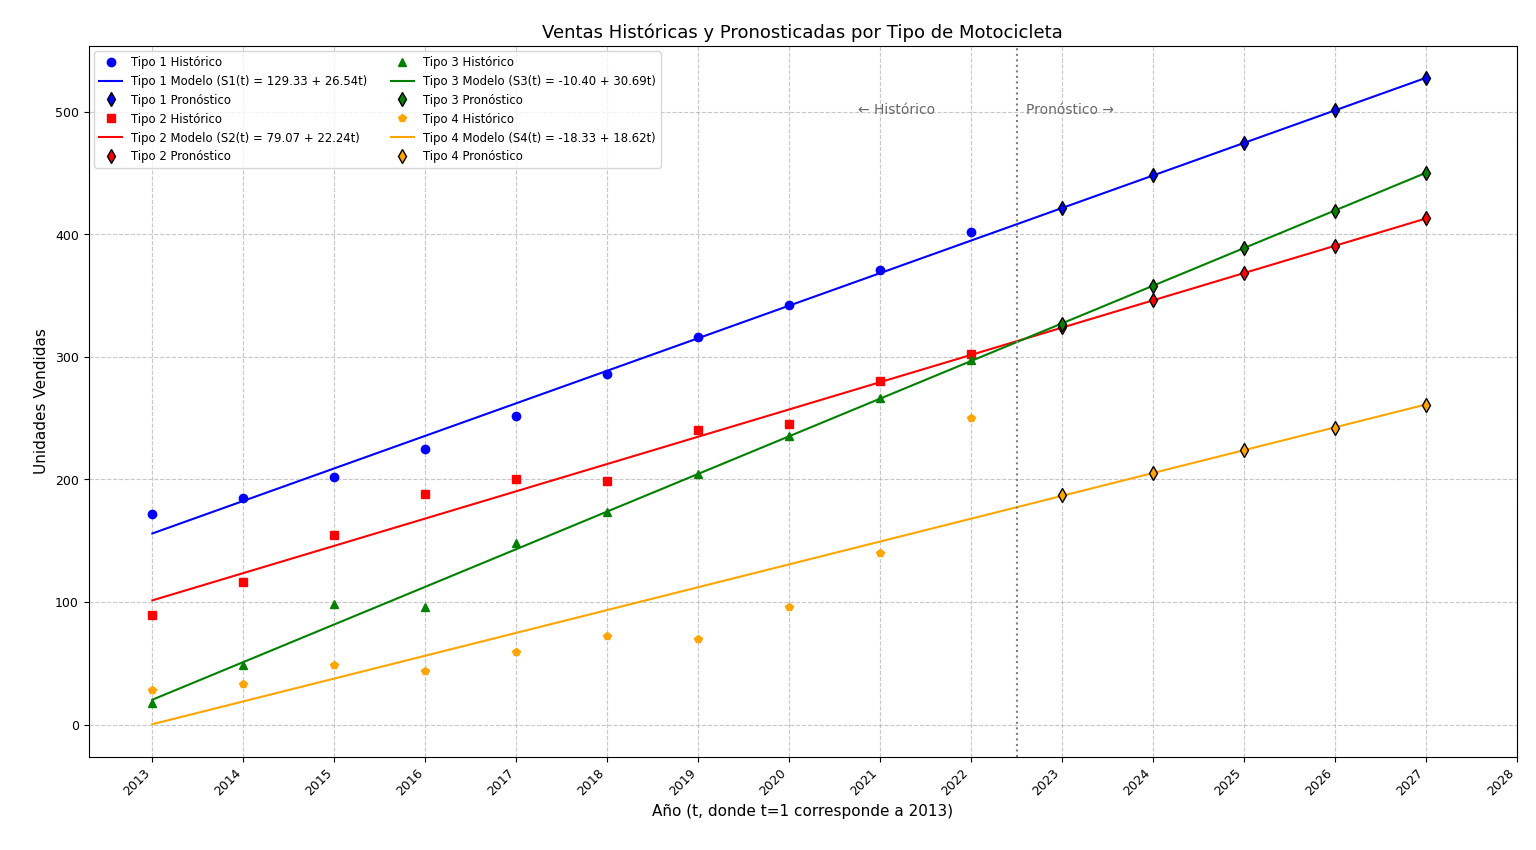
\includegraphics[width=0.7\linewidth]{Ventas historicas y pronosticadas por tipo moto.png}
\caption{Ventas históricas (2013–2022), modelos ajustados y pronósticos (2023–2027) por tipo de moto.}
\label{fig:ventas_combinada_img}
\end{figure}

\subsection{Estimación Inicial de Componentes}
Multiplicando la matriz $C$ por los vectores de ventas proyectadas para 2024 ($t=12$) y 2025 ($t=13$) (método \textit{directo}), se obtienen las necesidades mostradas en la Tabla~\ref{tab:componentes_directos}.

\begin{table}[H]
\tablesmall
\centering
\caption{Componentes requeridos (redondeado) para 2024 y 2025 (método directo).}
\label{tab:componentes_directos}
\begin{tabular}{@{}lrr@{}}
\toprule
Componente & Req. 2024 & Req. 2025 \\ \midrule
1  & 1152 & 1231 \\
2  & 1459 & 1561 \\
3  & 205  & 224  \\
4  & 205  & 224  \\
5  & 358  & 389  \\
6  & 2036 & 2158 \\
7  & 1832 & 1946 \\
8  & 3137 & 3330 \\
9  & 1510 & 1620 \\
10 & 794  & 842  \\ \bottomrule
\end{tabular}
\end{table}

\begin{figure}[H]
\centering
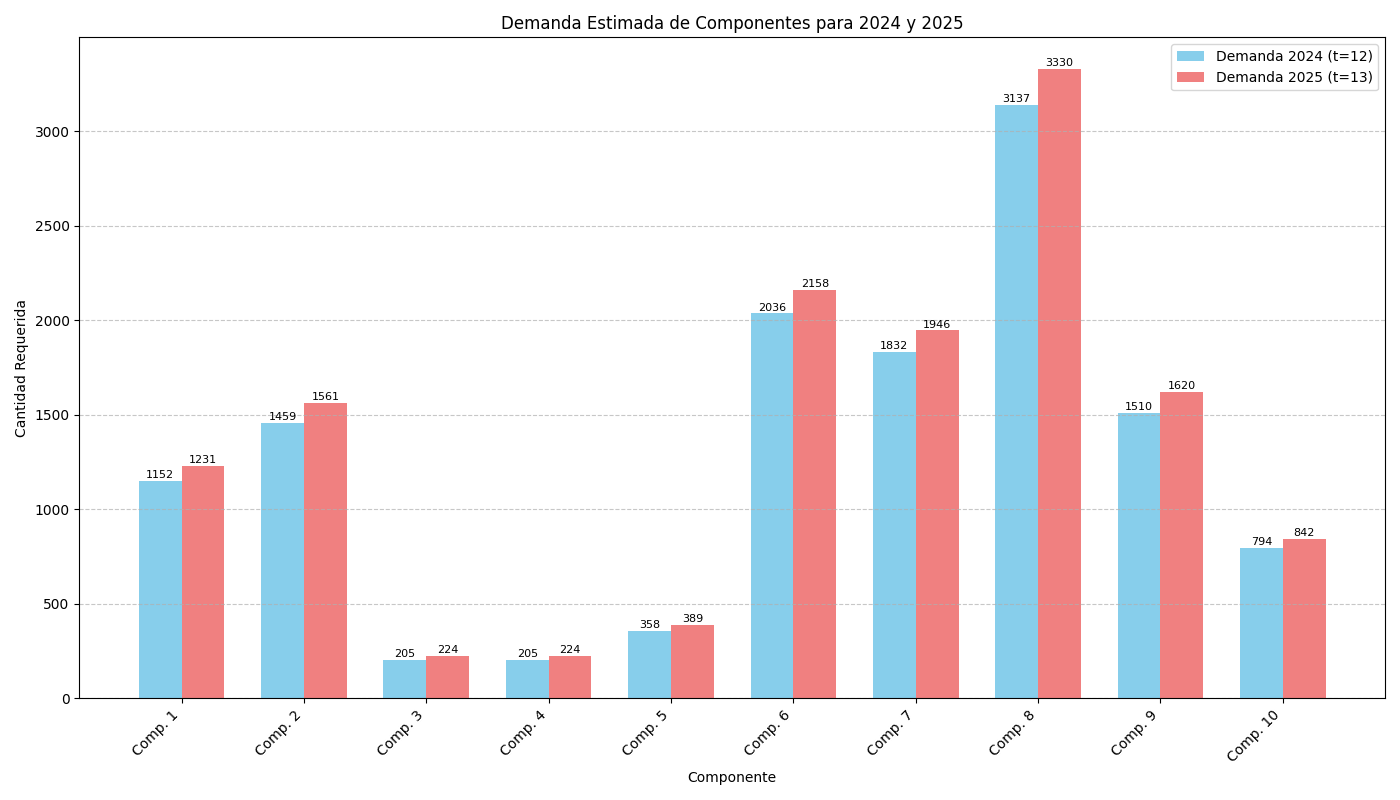
\includegraphics[width=0.7\linewidth]{Demanda estimada de componentes para 2024 y 2025.png}
\caption{Demanda estimada de componentes (método directo) para 2024 y 2025.}
\label{fig:demanda_componentes_2024_2025_img}
\end{figure}

\subsection{Modelo Global (Hiperplano)}
Se consideró un modelo lineal simple para las \textbf{ventas totales} $S_{\rm total}(t)$:
\[
S_{\rm total}(t) \;=\; \beta_0^{\rm tot} + \beta_1^{\rm tot}\,t,
\]
usando $t=1\dots10$ (2013–2022). Los coeficientes obtenidos (Python) son:
\[
\beta_0^{\rm tot} = 179.67,\quad \beta_1^{\rm tot} = 98.10,\quad
\text{ECM}_{\rm tot} = 1543.28,\quad R^2_{\rm tot} = 0.9809.
\]
Con este modelo se proyectan ventas totales:
\[
\begin{aligned}
2023\,(t=11):\;&1259\text{ unidades},\\
2024\,(t=12):\;&1357\text{ unidades},\\
2025\,(t=13):\;&1455\text{ unidades},\\
2026\,(t=14):\;&1553\text{ unidades},\\
2027\,(t=15):\;&1651\text{ unidades}.
\end{aligned}
\]
La Figura~\ref{fig:ajuste_global_hiperplano_img} muestra el ajuste histórico y la proyección.

\begin{figure}[H]
\centering
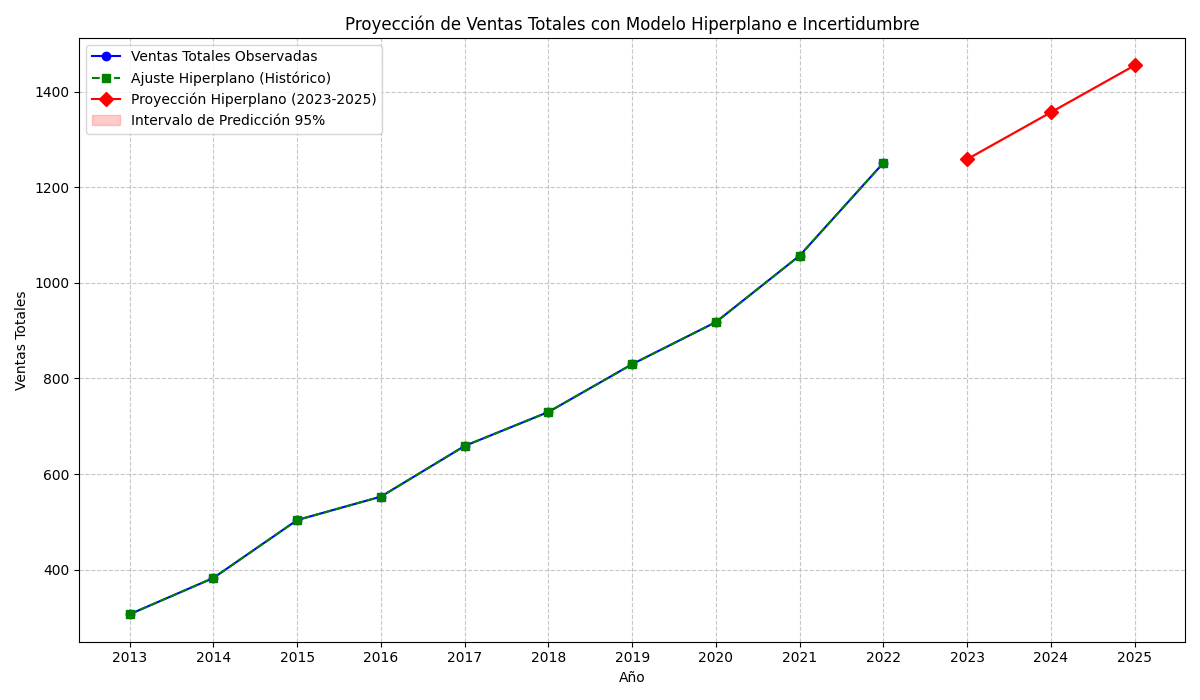
\includegraphics[width=0.7\linewidth]{Proyeccion de ventas totales con modelo hiperplano e incertidumbre.png}
\caption{Ventas totales observadas vs.\ predichas (modelo hiperplano) con banda de incertidumbre.}
\label{fig:ajuste_global_hiperplano_img}
\end{figure}

\subsection{Intervalos de Predicción (95\%)}
Para 2024 ($t=12$) y 2025 ($t=13$), el intervalo de predicción del 95\% se calculó con
\(\alpha=0.05\), grados de libertad $n-2=8$. Los resultados son:
\[
\begin{aligned}
2024: &\;1357\;[\;1242,\;1472\;],\;\text{margen} \pm115\;(8.5\%)\\
2025: &\;1455\;[\;1334,\;1576\;],\;\text{margen} \pm121\;(8.3\%)
\end{aligned}
\]
Estos intervalos reflejan la incertidumbre asociada al modelo global.

\subsection{Estimación Corregida de Componentes}
Para 2024 y 2025, en lugar de usar directamente los pronósticos individuales, se distribuyeron las ventas totales proyectadas según las \textbf{proporciones promedio históricas} de cada tipo:
\[
\text{Proporciones} = [0.405,\;0.288,\;0.201,\;0.106].
\]
Así, las ventas totales proyectadas asignadas a cada tipo son:
\[
\begin{aligned}
&2024:\,1357\times\text{proporciones} = [550,\;391,\;272,\;144]\;\text{(aprox.)},\\
&2025:\,1455\times\text{proporciones} = [589,\;419,\;292,\;155]\;\text{(aprox.)}.
\end{aligned}
\]
Multiplicando por $C$, obtenemos las \textbf{necesidades corregidas} (Tabla~\ref{tab:componentes_corregidos}).

\begin{table}[H]
\tablesmall
\centering
\caption{Demandas de componentes \textbf{corregidas} para 2024 y 2025.}
\label{tab:componentes_corregidos}
\begin{tabular}{@{}lrr@{}}
\toprule
Componente & Req. 2024 & Req. 2025 \\ \midrule
1  & 1213 & 1300 \\
2  & 1516 & 1625 \\
3  & 144  & 155  \\
4  & 144  & 155  \\
5  & 272  & 292  \\
6  & 2430 & 2606 \\
7  & 2112 & 2265 \\
8  & 3674 & 3939 \\
9  & 1485 & 1592 \\
10 & 940  & 1008 \\ \bottomrule
\end{tabular}
\end{table}

En total, los componentes requeridos son:
\[
\begin{aligned}
\text{Total 2024} &= 13\,930, \quad\text{media } = \frac{13\,930}{1357} \approx 10.3\ \text{componentes/moto},\\
\text{Total 2025} &= 14\,937, \quad\text{media } = \frac{14\,937}{1455} \approx 10.3\ \text{componentes/moto}.
\end{aligned}
\]

\subsection{Simulación de Monte Carlo (2024–2025)}
Se realizaron 10\,000 simulaciones asumiendo errores normales con $\sigma=\sqrt{\text{ECM}_{\rm tot}}\approx 39.3$. Para cada iteración se:
\begin{enumerate}
    \item Simularon ventas totales 2024 y 2025.
    \item Distribuyeron según proporciones históricas.
    \item Calculó demanda de componentes corregida.
\end{enumerate}
Los resultados más relevantes son:

\begin{itemize}\small
    \item \textbf{Ventas totales (MC):}
    \begin{itemize}\small
        \item 2024: media = 1357, IC 95\% = [1280, 1436], error relativo = ±5.7\%.
        \item 2025: media = 1455, IC 95\% = [1377, 1533], error relativo = ±5.4\%.
    \end{itemize}
    \item \textbf{Demanda de componentes (MC, 2024):}
    \begin{itemize}\small
        \item Componente 1: media = 1213, IC 95\% = [1144, 1283].
        \item Componente 2: media = 1516, IC 95\% = [1430, 1604].
        \item Componente 3: media = 144, IC 95\% = [136, 153].
        \item Componente 4: media = 144, IC 95\% = [136, 153].
        \item Componente 5: media = 272, IC 95\% = [257, 288].
        \item Componente 6: media = 2431, IC 95\% = [2293, 2572].
        \item Componente 7: media = 2113, IC 95\% = [1993, 2235].
        \item Componente 8: media = 3675, IC 95\% = [3466, 3888].
        \item Componente 9: media = 1485, IC 95\% = [1401, 1572].
        \item Componente 10: media = 941, IC 95\% = [887, 995].
    \end{itemize}
\end{itemize}

\section{Discusión}
\begin{itemize}\small
    \item Los modelos individuales para Tipos 1 y 3 muestran ajustes casi perfectos (R² = 0.99), mientras que Tipo 2 (R² = 0.97) y, especialmente, Tipo 4 (R² = 0.71) tienen mayor error. Esto indica que el modelo lineal simple es insuficiente para el Tipo 4.
    \item El modelo global de ventas totales ($R^2 = 0.9809$) confirma que la suma de las ventas individuales sigue una tendencia lineal fuerte. Su ECM de 1543.28 es coherente con la variabilidad conjunta.
    \item Los intervalos de predicción del 95\% (±8 %) para 2024–2025 muestran que, aunque la tendencia es clara, existe variabilidad significativa que debe incorporarse en la planificación de inventario.
    \item La estimación corregida de componentes—usando proporciones históricas—produce demandas ligeramente superiores al método directo, reflejando mejor la dinámica global de ventas. El promedio de 10.3 componentes por moto es consistente con la matriz $C$ y las proporciones históricas.
    \item La simulación de Monte Carlo reduce el error relativo de ventas totales a ±5–6 % y ajusta rangos de demanda de componentes a niveles más estrechos que el hiperplano solo, ofreciendo mayor confianza a la planificación.
\end{itemize}

\section{Conclusiones}
\begin{enumerate}\small
    \item \textbf{Coeficientes y ajuste de los modelos individuales:}
    \begin{itemize}
        \item Moto Tipo 1: $\beta_0 = 129.33$, $\beta_1 = 26.54$, ECM = 59.41, R² = 0.99. Ajuste excelente.
        \item Moto Tipo 2: $\beta_0 = 79.07$, $\beta_1 = 22.24$, ECM = 114.16, R² = 0.97. Buen ajuste, ligera variabilidad no explicada.
        \item Moto Tipo 3: $\beta_0 = -10.40$, $\beta_1 = 30.69$, ECM = 56.90, R² = 0.99. Ajuste excelente, intercepto negativo sin impacto en el rango de datos.
        \item Moto Tipo 4: $\beta_0 = -18.33$, $\beta_1 = 18.62$, ECM = 1174.68, R² = 0.71. Ajuste deficiente; tendencia lineal limitada.
    \end{itemize}

    \item \textbf{Pronósticos de ventas (2023–2027):}
    \[
    \begin{array}{lcccc}
    \text{Año (t)} & \text{Tipo 1} & \text{Tipo 2} & \text{Tipo 3} & \text{Tipo 4} \\ \midrule
    2023\,(11) & 421 & 324 & 327 & 187 \\
    2024\,(12) & 448 & 346 & 358 & 205 \\
    2025\,(13) & 474 & 368 & 389 & 224 \\
    2026\,(14) & 501 & 390 & 419 & 242 \\
    2027\,(15) & 527 & 413 & 450 & 261 \\
    \end{array}
    \]
    \begin{itemize}
        \item Tipo 1 y 3 lideran en unidades; Tipo 4 sigue siendo impredecible.
    \end{itemize}

    \item \textbf{Requerimientos de componentes (método directo) para 2024–2025:}
    \[
    \begin{array}{lcc}
    \text{Componente} & \text{Req.\ 2024} & \text{Req.\ 2025} \\ \midrule
    1  & 1152 & 1231 \\
    2  & 1459 & 1561 \\
    3  & 205  & 224  \\
    4  & 205  & 224  \\
    5  & 358  & 389  \\
    6  & 2036 & 2158 \\
    7  & 1832 & 1946 \\
    8  & 3137 & 3330 \\
    9  & 1510 & 1620 \\
    10 & 794  & 842  \\ \bottomrule
    \end{array}
    \]
    \begin{itemize}
        \item Verificación: Componente 1 en 2024 = 1152 (coincide con $R_{2024}$).
    \end{itemize}

    \item \textbf{Modelo global (hiperplano) para ventas totales:}
    \[
    S_{\text{total}}(t) = 179.67 + 98.10\,t, \quad \text{ECM}_{\text{tot}} = 1543.28,\ R^2_{\text{tot}} = 0.9809.
    \]
    \[
    \begin{aligned}
    2023\,(11): &\;1259,\\
    2024\,(12): &\;1357,\\
    2025\,(13): &\;1455,\\
    2026\,(14): &\;1553,\\
    2027\,(15): &\;1651.
    \end{aligned}
    \]

    \item \textbf{Intervalos de predicción (95 %):}
    \begin{itemize}
        \item 2024: 1357 [1242, 1472], margen ±115 (8.5 %).
        \item 2025: 1455 [1334, 1576], margen ±121 (8.3 %).
    \end{itemize}
    \begin{itemize}
        \item Indican volatilidad aun cuando la tendencia es lineal fuerte.
    \end{itemize}

    \item \textbf{Estimación corregida de componentes (2024–2025):}
    \[
    \text{Proporciones promedio} = [0.405,\;0.288,\;0.201,\;0.106].
    \]
    \[
    \begin{aligned}
    &\text{2024: reparto }[550,\,391,\,272,\,144],\quad \text{2025: }[589,\,419,\,292,\,155]. \\
    &\text{Demandas corregidas:}\\
    &\begin{array}{lcc}
    \text{Comp.} & \text{Req.\ 2024} & \text{Req.\ 2025} \\ \midrule
    1  & 1213 & 1300 \\
    2  & 1516 & 1625 \\
    3  & 144  & 155  \\
    4  & 144  & 155  \\
    5  & 272  & 292  \\
    6  & 2430 & 2606 \\
    7  & 2112 & 2265 \\
    8  & 3674 & 3939 \\
    9  & 1485 & 1592 \\
    10 & 940  & 1008 \\ \bottomrule
    \end{array}
    \end{aligned}
    \]
    \begin{itemize}
        \item Totales: 13 930 (2024), 14 937 (2025), promedio = 10.3 componentes/moto.
    \end{itemize}

    \item \textbf{Simulación Monte Carlo (10 000 iteraciones):}
    \begin{itemize}
        \item Ventas totales:
        \begin{itemize}
            \item 2024: media = 1357, IC 95 % = [1280, 1436], error ± 5.7 %.
            \item 2025: media = 1455, IC 95 % = [1377, 1533], error ± 5.4 %.
        \end{itemize}
        \item Demanda componentes 2024 (ejemplos):
        \[ \text{Comp.\ 1: media=1213, IC [1144, 1283]; Comp.\ 2: media=1516, IC [1430, 1604]; \dots} \]
        \item La simulación reduce la incertidumbre de componentes a ±5–6 % frente a ±8 % del hiperplano.
    \end{itemize}

    \item \textbf{Resumen ejecutivo:}
    \begin{itemize}
        \item El hiperplano explica 98.09 % de la variabilidad histórica (\(R^2=0.9809\)).
        \item Error estándar ≈ ± 39.3 unidades (ventas totales).
        \item Promedio de componentes por moto = 10.3 (coincide con \(C\) y proporciones históricas).
    \end{itemize}
\end{enumerate}

\section*{Anexo: Código Fuente}
El código Python completo (regresiones, pronósticos, cálculos de ECM/R², hiperplano, intervalos, Monte Carlo y gráficos) está disponible en:
\begin{center}
\url{https://github.com/Rojas-09/Trabajo-Lineal.git}
\end{center}

\end{document}

% Fin del documento
